\section{Empirical Application: Domestic Solar PV Adoption in England}\label{sec:solar}

% ---------------------------------------------------------------------------
\subsection{Motivation and data}\label{sec:solar_data}

The diffusion of rooftop solar photovoltaic (PV) systems displays the three features that motivate ZISAR.
First, adoption is spatially contagious: households are more likely to install panels when neighbours have done so, through visibility, word of mouth and local installer activity, as documented for the United States \citep{bollinger_gillingham2012,graziano_gillingham2015,kwan2012}, Germany \citep{rode_weber2016,dharshing2017,schaffer_brun2015} and the United Kingdom \citep{balta_ozkan2015,snape2016}.
Second, small-area counts contain zeros of two different kinds.
In neighbourhoods dominated by purpose-built blocks of flats, no household controls a roof and domestic installation is infeasible: these are \emph{structural} zeros.
In neighbourhoods of houses, a zero over a given period only means that no household happened to adopt: these are \emph{sampling} zeros of a positive-intensity process.
Third, intensities vary widely with income, tenure, housing stock and local markets, producing overdispersion.
The application therefore asks for both parts of the restricted model at once, the spatial parameter and the inflation process, and the direct and indirect effects of Section~\ref{sec:est_effects} are its quantities of interest.

\paragraph{Policy context and outcome.}
The Feed-in Tariff (FiT) scheme, opened in April 2010, paid British households a generation tariff for every kWh produced by small-scale renewable installations.
For domestic PV systems of up to 4\,kW the tariff was 41.3p/kWh at the start, was halved in 2012 and lowered in steps thereafter, and was cut by about two thirds, to 4.39p/kWh, from 8~February 2016; the scheme closed to new applicants in March 2019.
We study the boom that preceded the cut.
In England the scheme accredited about 19{,}000 domestic PV systems of up to 10\,kW in 2010, 158{,}000 in 2011, 125{,}000 in 2012, 75{,}000 in 2013, 103{,}000 in 2014 and 133{,}000 in 2015, against about 20{,}000 a year after the cut.

The window matters for the separation of the two kinds of zeros.
After almost six years of generous tariffs, adoption had reached nearly every neighbourhood where it was feasible: in an area of some 650 households for which the count process predicts tens of installations, a zero is improbable unless installation is infeasible, and the zeros that remain are informative about the housing stock.
After the cut adoption became sparse, and a third of the areas record no installation between 8~February 2016 and March 2019, most of them areas that had adopted before; with intensities of one or two installations per area a zero says little about feasibility, and a spatially dependent count process reproduces clusters of such zeros as sampling zeros.
We therefore model the boom and use the installations after the cut only to validate the structural zeros (Section~\ref{sec:solar_results}).

The outcome is taken from the Ofgem Central FiT Register (installation report of 30~June 2026), which lists every accredited installation with its technology, type, capacity, commissioning date and Lower-layer Super Output Area (LSOA).
We count the domestic PV installations of up to 10\,kW commissioned before 8~February 2016, excluding extensions of existing systems: 611{,}903 installations, of which 4{,}888 were commissioned before April 2010 and joined the scheme when it opened.
The limit of 10\,kW, the upper limit of the second FiT tariff band, keeps the rooftop systems of single houses (typically 2--4\,kW) and leaves out 7{,}089 larger domestic systems (1.1\%).
The register does not geocode 2.4\% of the domestic installations of the window.

The units are the LSOAs of England, small statistical areas of 400--1{,}200 households designed to be socially homogeneous.
The register geocodes installations to the 2001 LSOAs, whereas the 2011 Census and the Indices of Deprivation use the 2011 LSOAs.
For 97\% of the areas the two coincide; where an LSOA was split or merged between the two censuses we aggregate the areas linked by the official best-fit lookup into a single unit, obtaining $n = 32{,}322$ units with a median of 650 households.
The harmonisation matters for a zero-inflated model: matching the register to the 2011 codes directly would assign zero installations to every one of the 1{,}172 LSOAs created in 2011, a spurious excess of zeros.

The number of installations per unit has mean 18.9, variance 396, median 13 and maximum 308; 1{,}112 units (3.4\%) record none and 1{,}323 record one.
Zeros concentrate where the housing stock leaves no roofs to equip: 24\% of the units in the top decile of the share of flats record no installation, against 0.6\% of the units below the median share, and 514 of the 1{,}153 units where flats make up more than 80\% of the household spaces record none.
Greater London has 15\% of the units and 815 of the zeros (73\%): 17\% of its units record no installation, against 1.1\% elsewhere.
The zeros persist after the cut: 873 of the 1{,}112 units without an installation in the boom still had none in March 2019.

\paragraph{Covariates and spatial weights.}
The covariates describe slow-moving characteristics of the areas, measured within the window, and are standardised (Table~\ref{tab:solar_desc}).
The count process includes eleven covariates of its own.
Five are socio-economic: the shares of social-rented households, of residents in managerial and professional occupations (NS-SEC classes 1--2), of residents aged 65 and over and of households with dependent children, from the 2011 Census, and the income-deprivation rate of the English Indices of Deprivation 2019.
Five describe housing and energy: the number of households (log); the share of detached houses; the share of dwellings in Council Tax bands E--H, a measure of property value from the Valuation Office Agency (VOA) stock of properties in 2015; the share of households without gas central heating, who face higher energy costs; and the mean domestic electricity consumption per meter in 2010 (log), from the Department for Energy Security and Net Zero, measured at the start of the scheme because later consumption is net of the panels' self-consumption.
The last is the northing of the population-weighted centroid, which captures the decline of solar irradiation with latitude.

The inflation process includes six variables that can make domestic installation infeasible: the share of household spaces in flats, population density (log) and the shares of private-rented households, of residents in communal establishments such as student halls and care homes, of household spaces with no usual resident and of dwellings built before 1919 (VOA).
These six also enter the count process, since the housing stock shifts the number of eligible roofs even where installation is feasible; their effects on $\E[\by]$ therefore combine the count channel \eqref{eq:effects_count} and the inflation channel \eqref{eq:effects_zero_channel}.

\begin{table}[htbp]
\centering
\caption{Descriptive statistics of the outcome and covariates ($n = 32{,}322$ units). Shares and rates in per cent unless stated; VOA counts are rounded to the nearest ten, so that VOA shares can slightly exceed 100. Sources: Ofgem Central FiT Register; 2011 Census; English Indices of Deprivation 2019; VOA Council Tax stock of properties 2015; DESNZ sub-national electricity consumption 2010.}\label{tab:solar_desc}
\small
\begin{tabular}{lrrrrr}
\toprule
 & Mean & SD & Min & Median & Max \\
\midrule
Domestic PV installations to 7 Feb 2016 & 18.93 & 19.89 & 0 & 13 & 308 \\
\midrule
\multicolumn{6}{l}{\textit{Count process}} \\
\quad Social-rented households & 17.4 & 17.2 & 0.0 & 11.2 & 92.5 \\
\quad Income-deprivation rate & 12.9 & 9.4 & 0.3 & 10.0 & 60.9 \\
\quad Managerial and professional (NS-SEC 1--2) & 31.2 & 12.2 & 2.7 & 30.4 & 78.5 \\
\quad Aged 65 and over & 16.8 & 7.1 & 0.4 & 16.2 & 60.7 \\
\quad Households with dependent children & 29.7 & 7.9 & 2.4 & 29.2 & 72.9 \\
\quad Households (number) & 682.6 & 171.0 & 304 & 650 & 6304 \\
\quad Detached houses & 22.8 & 21.8 & 0.0 & 13.8 & 97.2 \\
\quad Council Tax bands E--H & 18.8 & 23.0 & 0.0 & 8.8 & 102.0 \\
\quad Without gas central heating & 20.3 & 17.9 & 1.6 & 14.6 & 98.7 \\
\quad Electricity per meter, 2010 (kWh) & 4178 & 899 & 1462 & 3982 & 13360 \\
\quad Northing (km) & 276.7 & 127.4 & 10.6 & 260.9 & 654.4 \\
\midrule
\multicolumn{6}{l}{\textit{Inflation and count processes}} \\
\quad Flats (share of household spaces) & 20.0 & 22.2 & 0.0 & 11.6 & 99.7 \\
\quad Population density (per km$^2$) & 4225 & 4154 & 3 & 3430 & 68470 \\
\quad Private-rented households & 16.0 & 11.3 & 1.3 & 12.2 & 87.9 \\
\quad Residents in communal establishments & 1.5 & 4.6 & 0.0 & 0.0 & 86.7 \\
\quad Household spaces with no usual resident & 3.9 & 3.5 & 0.0 & 3.1 & 71.4 \\
\quad Dwellings built before 1919 & 20.8 & 24.3 & 0.0 & 11.3 & 101.4 \\
\bottomrule
\end{tabular}
\end{table}

The spatial weights matrix $\bW$ is the row-standardised queen-contiguity matrix of the generalised (20\,m) LSOA boundaries, with on average 5.86 neighbours per unit; the Isles of Scilly, the only unit without contiguous neighbours, are linked to the nearest unit.
Because $n = 32{,}322$ rules out the dense eigendecomposition, the log-determinant is computed by sparse Cholesky factorisation \eqref{eq:logdet_sparse}.

% ---------------------------------------------------------------------------
\subsection{Estimates}\label{sec:solar_results}

We estimate six specifications.
Three are the benchmarks of the Monte~Carlo study: the negative binomial (NB) regression, the zero-inflated NB (ZINB) and the SAR-NB with the spatial lag $\bW\by$ instrumented by $[\bX,\bW\bX,\bW^2\bX]$.
Three are fitted with the ZISAR template, by the algorithm of Section~\ref{sec:est_algorithm} and the log-determinant \eqref{eq:logdet_sparse}: the restricted ZISAR; the ZINB with Gaussian random effects (ZINB-RE), obtained by fixing $\rho = 0$; and the spatial NB with random effects and no zero-inflation (SAR-NB-RE), obtained by fixing the inflation intercept at $-20$ and its slopes at zero, so that $\pi_i \approx 2\times 10^{-9}$.
The last two are nested in ZISAR, and each removes one of its two parts: the comparison with the ZINB-RE measures what the spatial parameter adds, the comparison with the SAR-NB-RE what the inflation process adds.
A ZISAR fit takes five to six minutes on a laptop (Apple M5 Pro), the effects decomposition under a minute and the bootstrap about two hours on three cores.

\paragraph{Numerical behaviour and inference.}
Started from the default values, the optimiser stops 33 log-likelihood points below the optimum it reaches when started from the SAR-NB-RE estimates, which we report.
At that optimum it stops without declaring convergence, with a largest gradient component of order $10^8$, and the Hessian is not a reliable basis for standard errors.
The cause is the combination of structural zeros with high intensities.
For a unit with no installation whose covariates predict tens, the conditional distribution of $\eta_i$ given $y_i = 0$ has two modes: one near the value implied by the covariates and the neighbours, where the zero is structural, and one far below it, where the zero is a sampling zero of a unit with a very low intensity.
The inner maximisation picks one of them, and where the two have nearly the same height a small change in $\btheta$ makes it switch, so that $\ell_{\mathrm{LA}}$ is not smooth there and the quasi-Newton iterations stall.
A large gradient at the stopping point is also the symptom of the spurious optima that the unit-level field of the general model produces (Appendix~\ref{app:general}), so we check by simulation that this optimum is genuine.
On a data set simulated from the fitted SAR-NB-RE, which has no structural zeros, ZISAR converges without difficulty (largest gradient component 0.7) and estimates 6 structural zeros, with a likelihood-ratio statistic for $\pi_i = 0$ of 0.6.
On a data set simulated from the fitted ZISAR it stops with the same large gradient, but recovers the structural zeros (518 estimated against 511 expected) and the spatial parameter ($\hat\rho = 0.668$ against 0.633), with a likelihood-ratio statistic of 761.
The large gradient thus accompanies structural zeros among units of high intensity, and does not signal a spurious optimum.
For inference we use a parametric bootstrap: $B = 30$ data sets are simulated from the fitted ZISAR and each is refitted from the estimates; the standard errors of the parameters and of the effects are the standard deviations of the replicates.
Only 5 of the 30 replicate fits converge formally, with a median largest gradient component of $7\times 10^7$, yet they show no bias in the quantities of interest: they average $\hat\rho = 0.633$ (range 0.614--0.647) and 511 structural zeros (472--588), the values of the fitted model.
The bootstrap standard errors are close to the Hessian ones for the count process and larger for the inflation process: 0.153 against 0.083 for its intercept and 0.079 against 0.050 for the share of flats.
Because each replicate starts from the estimates, they measure the sampling variability around the reported optimum.
Started from the default values, the fit of the simulated data set above stopped at $\hat\rho = 0.668$, $\hat\sigma = 0.44$ and $\hat\kappa = 20$: the optimiser can stop at different points of the ridge between $\rho$, $\sigma$ and $\kappa$, a source of variation that the bootstrap does not include.

Table~\ref{tab:solar_estimates} reports the estimates of the four main specifications and Table~\ref{tab:solar_fit} the fit of all six.

\begin{table}[htbp]
\centering
\caption{Estimates for domestic PV installations commissioned before 8~February 2016 ($n=32{,}322$ units). Covariates standardised; standard errors in parentheses, from the parametric bootstrap ($B = 30$) for ZISAR. The SAR-NB coefficient on $\widehat{\bW\by}$ (in brackets) multiplies the observed neighbourhood count in the log-mean and is not on the scale of $\rho$. For ZISAR, $\kappa$ is at the upper bound of the optimisation box.}\label{tab:solar_estimates}
\footnotesize
\begin{tabular}{lrrrr}
\toprule
 & NB & ZINB & SAR-NB & ZISAR \\
\midrule
\multicolumn{5}{l}{\textit{Count process} ($\bbeta$)} \\
Intercept                          & $2.693$ (0.004) & $2.712$ (0.004) & $2.128$ (0.015) & $0.895$ (0.016) \\
Social rented                      & $0.216$ (0.010) & $0.226$ (0.010) & $0.135$ (0.010) & $0.019$ (0.006) \\
Income deprivation                 & $0.063$ (0.010) & $0.036$ (0.010) & $0.101$ (0.010) & $0.031$ (0.008) \\
Managerial (NS-SEC 1--2)           & $0.034$ (0.009) & $0.019$ (0.009) & $0.030$ (0.009) & $-0.017$ (0.008) \\
Aged 65 and over                   & $0.006$ (0.008) & $-0.004$ (0.008) & $-0.019$ (0.008) & $-0.019$ (0.005) \\
Dependent children                 & $-0.127$ (0.007) & $-0.117$ (0.008) & $-0.112$ (0.007) & $-0.062$ (0.005) \\
Households (log)                   & $0.201$ (0.005) & $0.194$ (0.005) & $0.171$ (0.005) & $0.146$ (0.004) \\
Detached houses                    & $0.283$ (0.007) & $0.303$ (0.007) & $0.151$ (0.008) & $0.160$ (0.006) \\
Council Tax bands E--H             & $-0.169$ (0.008) & $-0.159$ (0.008) & $-0.074$ (0.008) & $-0.024$ (0.005) \\
Without gas central heating        & $0.029$ (0.007) & $0.057$ (0.007) & $-0.057$ (0.007) & $0.015$ (0.005) \\
Electricity per meter, 2010 (log)  & $-0.012$ (0.008) & $-0.041$ (0.009) & $0.062$ (0.009) & $0.009$ (0.007) \\
Northing                           & $-0.043$ (0.005) & $-0.037$ (0.004) & $-0.007$ (0.005) & $-0.010$ (0.003) \\
Flats                              & $-0.537$ (0.009) & $-0.461$ (0.010) & $-0.381$ (0.010) & $-0.162$ (0.008) \\
Density (log)                      & $-0.173$ (0.007) & $-0.167$ (0.007) & $-0.067$ (0.008) & $-0.056$ (0.005) \\
Private rented                     & $-0.064$ (0.009) & $-0.087$ (0.009) & $-0.081$ (0.009) & $-0.106$ (0.006) \\
Communal establishments            & $0.023$ (0.005) & $0.021$ (0.005) & $0.021$ (0.005) & $0.006$ (0.004) \\
No usual resident                  & $0.048$ (0.005) & $0.046$ (0.005) & $0.012$ (0.005) & $-0.003$ (0.004) \\
Built before 1919                  & $-0.145$ (0.006) & $-0.149$ (0.006) & $-0.116$ (0.006) & $-0.052$ (0.005) \\
$\rho$                             & --- & --- & [$0.028$ (0.001)] & $0.633$ (0.006) \\
\midrule
\multicolumn{5}{l}{\textit{Inflation process} ($\bgamma$)} \\
Intercept                          & --- & $-7.472$ (0.264) & --- & $-6.881$ (0.153) \\
Flats                              & --- & $1.783$ (0.128) & --- & $1.768$ (0.079) \\
Density (log)                      & --- & $1.512$ (0.239) & --- & $0.832$ (0.100) \\
Private rented                     & --- & $-0.238$ (0.075) & --- & $-0.247$ (0.070) \\
Communal establishments            & --- & $0.034$ (0.039) & --- & $0.018$ (0.054) \\
No usual resident                  & --- & $0.010$ (0.075) & --- & $0.097$ (0.059) \\
Built before 1919                  & --- & $-0.518$ (0.092) & --- & $-0.682$ (0.078) \\
\midrule
$\kappa$ (NB shape)                & $2.246$ & $2.363$ & $2.369$ & $500$ \\
$\sigma$ (RE std.\ dev.)           & --- & --- & --- & $0.497$ (0.003) \\
\bottomrule
\end{tabular}
\end{table}

\paragraph{Spatial dependence and structural zeros.}
ZISAR estimates $\hat\rho = 0.633$ (SE 0.006): the latent propensity to adopt of a unit depends strongly on that of its neighbours, and the spatial multiplier $1/(1-\hat\rho) = 2.7$ almost triples the effect of a uniform change in the covariates.
The likelihood-ratio statistic for $\rho = 0$, against the ZINB-RE, is 8{,}463, and the bootstrap $z$ statistic on $\tilde\rho$ is 73.
The spatial lag of the SAR-NB is also significant, and it lowers the AIC of the NB by 1{,}485 points, against 8{,}462 for the latent SAR over the ZINB-RE: an instrumented lag of observed counts captures a small part of the dependence.

The inflation process is driven by housing form.
The probability of a structural zero rises with the share of flats ($\hat\gamma = 1.77$) and with density ($0.83$) and, given these, is lower where the stock was built before 1919 ($-0.68$), which is consistent with old terraced houses, each with a roof of its own, as opposed to purpose-built blocks, and where private renting is more common ($-0.25$); communal establishments and vacant dwellings have no significant role.
The fitted probabilities are very skewed: the median $\hat\pi_i$ is 0.0008 and the 99th percentile 0.45; they average less than 0.003 in each of the first four quintiles of the share of flats and 0.075 in the fifth.
The model expects 511 structural zeros, 46\% of the 1{,}112 observed, and 463 observed zeros have a posterior probability of being structural above one half.
The structural zeros are concentrated in the urban cores: 75\% of them are in Greater London, and 236 of the 245 units with $\hat\pi_i > 0.5$ are there (Figure~\ref{fig:solar_maps}).

The posterior probability that an observed zero is structural, $P(s_i = 1\mid y_i=0) = \hat\pi_i/[\hat\pi_i + (1-\hat\pi_i)\,h(0;\hat\eta_i,\hat\kappa)]$, can be checked against information the model does not use, namely the installations made after the cut.
A unit without suitable roofs should remain without installations once the tariff falls, whereas a sampling zero of the boom may adopt later.
Among the boom zeros, the posterior probability averages 0.46 for the 873 units still without an installation in March 2019 and 0.28 for the 239 that adopted after the cut.
Ranked by the posterior, the third of the zeros with the lowest values made 0.80 installations per unit after the cut, the middle third 0.28 and the top third 0.18, and the share still at zero rises from 68\% to 80\% and 87\%.
As a classifier of the units that remain at zero, the posterior probability has an area under the ROC curve of 0.63.
The check is conservative: after the cut adoption fell by more than four fifths, so that most sampling zeros of the boom also stay at zero.

\begin{figure}[htbp]
\centering
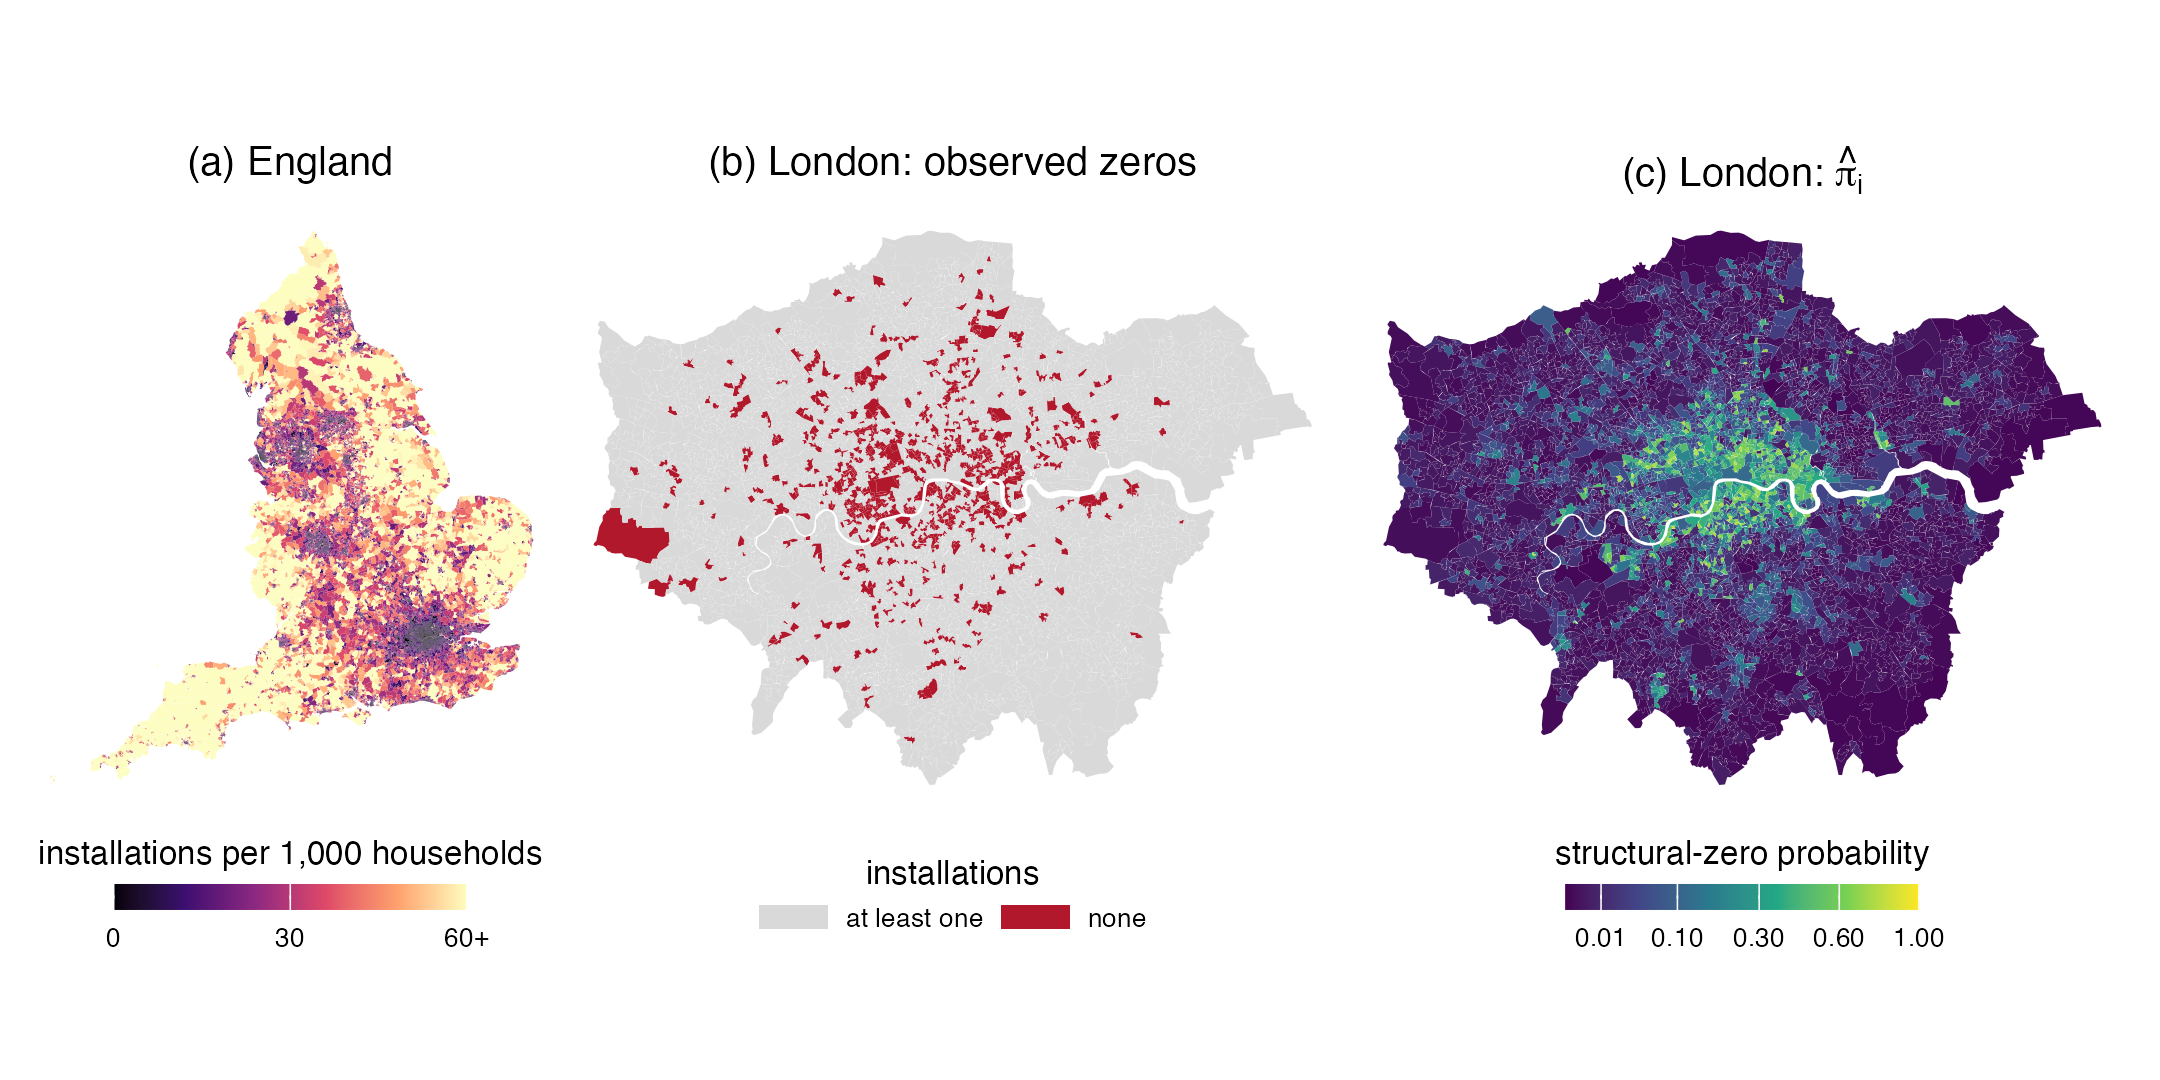
\includegraphics[width=\textwidth]{figures/solar_boom_maps.png}
\caption{(a) Domestic PV installations per 1{,}000 households commissioned before 8~February 2016. (b) London units with no installation in the window. (c) Estimated probability of a structural zero, $\hat\pi_i$, in London: the model assigns a high probability of a structural zero to the inner areas where flats prevail.}\label{fig:solar_maps}
\end{figure}

\paragraph{Covariate effects and dispersion.}
The coefficients of ZISAR are smaller than those of the aspatial models because they act on the latent predictor before the multiplier; the effects of Table~\ref{tab:solar_effects} are the comparable quantities.
More informative is what changes in relative terms.
The share of social-rented households has a large positive coefficient in the NB and the ZINB (0.216 and 0.226) and the share of dwellings in the upper Council Tax bands a large negative one ($-0.169$ and $-0.159$).
The nested models show where the change comes from: both are still large with independent random effects (0.130 and $-0.179$ in the ZINB-RE) and both shrink by an order of magnitude once the field is spatial (0.020 and $-0.024$ in the SAR-NB-RE, 0.019 and $-0.024$ in ZISAR).
Tenure and property value are spatially clustered, and so is adoption: a model without a spatial field reads the common clustering as an effect of the covariates.
In the same way the coefficients of detached houses and of households with dependent children are halved, and those of managerial occupations and of the elderly share turn from positive to negative.
In ZISAR adoption is higher where there are more households and more detached houses, and lower where flats, private renting, density, pre-1919 dwellings and households with dependent children are more common; it declines from south to north, as does the solar resource.
Given the housing stock, it is also somewhat higher where social renting and income deprivation are more common and lower in the upper Council Tax bands and where managerial occupations prevail, a pattern consistent with the programmes through which social landlords fitted panels to many homes at a time during the boom.

The models without a latent field attribute all the extra-Poisson variation to the NB shape ($\hat\kappa \approx 2.3$).
Once the field is spatial, the shape estimate runs to the upper bound of the optimisation box ($\kappa = 500$), in ZISAR as in the SAR-NB-RE, and the count distribution is effectively Poisson conditional on $\boldsymbol\eta$: the overdispersion is accounted for by the log-normal heterogeneity, $\hat\sigma = 0.497$, filtered through the spatial multiplier.
This is the trade-off between $\sigma^2$ and $\kappa^{-1}$ noted in the Monte~Carlo study, resolved here in favour of the Gaussian component.

\paragraph{Fit and residual dependence.}
Both parts of ZISAR are needed (Table~\ref{tab:solar_fit}).
Adding zero-inflation to the NB lowers the AIC by 1{,}051 points, adding random effects to the ZINB by a further 3{,}140, and making the field spatial by 8{,}462.
Zero-inflation remains relevant when the spatial field is present: ZISAR improves on the SAR-NB-RE by 538 AIC points and 479 BIC points (the likelihood-ratio statistic is 552 on seven restrictions, although the restriction $\pi_i = 0$ lies on the boundary of the parameter space and the $\chi^2_7$ reference is only indicative; the simulation above puts the statistic near zero when there are no structural zeros).
ZISAR has the lowest AIC and BIC of the six specifications, and neither nested model comes close to it.
The three models without zero-inflation under-predict the zeros by about a fifth (887--908 expected against 1{,}112 observed), whereas the zero-inflated ones come close or over-predict (1{,}123 for the ZINB-RE, 1{,}211 for ZISAR and 1{,}269 for the ZINB).

\begin{table}[htbp]
\centering
\caption{Fit of the six specifications and expected number of units with no installation (observed: 1{,}112). Expected zeros are marginal: for the random-effects models the latent field is integrated out by simulation from the fitted distribution (200 draws).}\label{tab:solar_fit}
\small
\begin{tabular}{lrrrrr}
\toprule
 & Log-lik. & $k$ & AIC & BIC & Expected zeros \\
\midrule
NB        & $-117{,}246$ & 19 & $234{,}531$ & $234{,}690$ & $902$ \\
ZINB      & $-116{,}714$ & 26 & $233{,}480$ & $233{,}697$ & $1{,}269$ \\
SAR-NB    & $-116{,}503$ & 20 & $233{,}046$ & $233{,}214$ & $887$ \\
ZINB-RE   & $-115{,}143$ & 27 & $230{,}340$ & $230{,}566$ & $1{,}123$ \\
SAR-NB-RE & $-111{,}187$ & 21 & $222{,}416$ & $222{,}592$ & $908$ \\
ZISAR     & $-110{,}911$ & 28 & $221{,}878$ & $222{,}113$ & $1{,}211$ \\
\bottomrule
\end{tabular}
\end{table}

Moran's $I$ of the counts is 0.550 ($z = 164$ under the normal approximation), and the Pearson residuals of the NB, the ZINB and the SAR-NB retain most of it ($I = 0.34$, $z = 101$--$103$): the covariates and the instrumented lag leave the spatial structure of adoption in the residuals.
The predicted innovations of ZISAR, $\hat\bu = (\mathbf{I}_n-\hat\rho\bW)\hat{\boldsymbol\eta} - \bX\hat\bbeta$, keep a small positive autocorrelation ($I = 0.08$): the latent field absorbs most of the dependence.

% ---------------------------------------------------------------------------
\subsection{Effects decomposition}\label{sec:solar_effects}

Because $\hat\rho$ is large, a coefficient of ZISAR does not measure the effect of its covariate: a change in one unit propagates to its neighbours through the latent field and returns.
Table~\ref{tab:solar_effects} reports the average direct, indirect and total effects on the expected number of installations of a one-standard-deviation increase in each covariate, computed as in Section~\ref{sec:est_effects}, with bootstrap standard errors.
For the six covariates that enter both processes the direct effect includes the inflation channel \eqref{eq:effects_zero_channel}, reported separately in the last column.

\begin{table}[htbp]
\centering
\caption{Average direct, indirect and total effects on the expected number of installations per unit (mean 18.9) of a one-standard-deviation increase in each covariate (ZISAR). Bootstrap standard errors ($B = 30$) in parentheses. The last column is the part of the direct effect that runs through the inflation probability.}\label{tab:solar_effects}
\footnotesize
\begin{tabular}{lrrrr}
\toprule
 & Direct & Indirect & Total & Inflation \\
\midrule
Social rented                      & $0.39$ (0.13) & $0.58$ (0.20) & $0.97$ (0.33) & --- \\
Income deprivation                 & $0.64$ (0.17) & $0.94$ (0.24) & $1.59$ (0.41) & --- \\
Managerial (NS-SEC 1--2)           & $-0.36$ (0.16) & $-0.52$ (0.24) & $-0.88$ (0.40) & --- \\
Aged 65 and over                   & $-0.40$ (0.11) & $-0.59$ (0.16) & $-1.00$ (0.27) & --- \\
Dependent children                 & $-1.29$ (0.11) & $-1.88$ (0.16) & $-3.17$ (0.27) & --- \\
Households (log)                   & $3.05$ (0.09) & $4.46$ (0.16) & $7.50$ (0.24) & --- \\
Detached houses                    & $3.33$ (0.13) & $4.87$ (0.22) & $8.19$ (0.34) & --- \\
Council Tax bands E--H             & $-0.51$ (0.12) & $-0.74$ (0.17) & $-1.25$ (0.28) & --- \\
Without gas central heating        & $0.31$ (0.10) & $0.46$ (0.15) & $0.77$ (0.25) & --- \\
Electricity per meter, 2010 (log)  & $0.19$ (0.14) & $0.27$ (0.21) & $0.46$ (0.35) & --- \\
Northing                           & $-0.21$ (0.06) & $-0.31$ (0.09) & $-0.51$ (0.15) & --- \\
\midrule
Flats                              & $-3.49$ (0.17) & $-4.95$ (0.27) & $-8.43$ (0.43) & $-0.102$ (0.004) \\
Density (log)                      & $-1.22$ (0.10) & $-1.72$ (0.14) & $-2.94$ (0.24) & $-0.048$ (0.007) \\
Private rented                     & $-2.21$ (0.12) & $-3.25$ (0.18) & $-5.45$ (0.30) & $0.014$ (0.004) \\
Communal establishments            & $0.13$ (0.08) & $0.19$ (0.11) & $0.32$ (0.19) & $-0.001$ (0.003) \\
No usual resident                  & $-0.07$ (0.09) & $-0.10$ (0.13) & $-0.17$ (0.22) & $-0.006$ (0.003) \\
Built before 1919                  & $-1.04$ (0.10) & $-1.58$ (0.15) & $-2.62$ (0.25) & $0.039$ (0.005) \\
\bottomrule
\end{tabular}
\end{table}

Indirect effects are the larger part: they account for 59\% of the total effect of every covariate that enters only the count process, a share fixed by $\hat\rho$ and by the weighting of the units by their fitted intensity, and for 58--60\% of the total effect of the other six.
A one-standard-deviation increase in the number of households (log) in every unit raises expected installations by 7.5 per unit, two fifths of the mean, of which 3.0 occurs through the unit's own latent propensity and 4.5 through the feedback from its neighbours; for the share of detached houses the total is 8.2, of which 3.3 is direct.
The share of flats has the largest negative effect ($-8.4$), followed by private renting ($-5.5$), households with dependent children ($-3.2$), density ($-2.9$) and pre-1919 dwellings ($-2.6$).
The inflation channel is small on average, because structural zeros are rare outside the urban cores; it is largest for the share of flats, $-0.10$ out of a direct effect of $-3.49$.
All total effects are distinguishable from zero at the 5\% level except those of electricity consumption, communal establishments and vacant dwellings.
A model with $\rho = 0$ has no indirect effects: the ZINB-RE would report the direct column alone, and the aspatial models a single coefficient per covariate, with the effects of social renting and property value an order of magnitude larger.

The estimate of $\rho$ measures how strongly the latent adoption propensities of neighbouring areas move together, given the covariates.
Peer effects of the kind documented by \citet{bollinger_gillingham2012} and \citet{graziano_gillingham2015} generate such dependence, but so do spatially correlated unobservables---the reach of local installers, roof orientation and shading, local campaigns---and a cross-section cannot separate the two \citep{manski1993,gibbons_overman2012}.
What the application establishes is narrower and, for inference on the covariates, sufficient: treating adoption as spatially independent, or ignoring the structural zeros, distorts the estimated role of tenure, property value, household composition and housing form, leaves strong dependence in the residuals and hides the larger part of every effect.

The restricted model suffices here: the structural zeros follow the housing stock, which the covariates of the inflation process measure.
A spatial field in the inflation predictor would be needed only if the structural zeros clustered beyond what these covariates explain; Appendix~\ref{app:general} shows how such a field can be estimated.
